\usetikzlibrary{arrows.meta,calc}
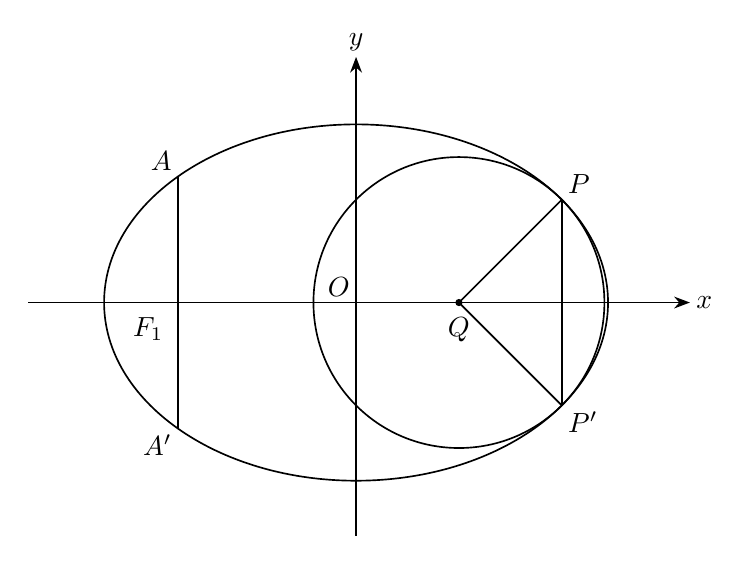
\begin{tikzpicture}[x=0.8cm,y=0.8cm,line width=.6pt,font=\normalsize,>=Stealth,
  label/.style={inner sep=2pt}]
\coordinate (O) at (0,0);
\coordinate (F1) at (-2.8284271247,0);
\coordinate (A) at (-2.8284271247,2);
\coordinate (Ap) at (-2.8284271247,-2);
\coordinate (Q) at (1.6329931620,0);
\coordinate (P) at (3.2659863240,1.6329931620);
\coordinate (Pp) at (3.2659863240,-1.6329931620);
\draw[->] (-5.2,0)--(5.3,0) node[label,right] {$x$};
\draw[->] (0,-3.7)--(0,3.9) node[label,above] {$y$};
\draw (O) ellipse[x radius=4,y radius=2.8284271247];
\draw (Q) circle[radius=2.3094010768];
\draw (A)--(Ap);
\draw (P)--(Pp);
\draw (Q)--(P);
\draw (Q)--(Pp);
\fill (Q) circle[radius=1.3pt];
\node[label,above left] at (A) {$A$};
\node[label,below left] at (Ap) {$A'$};
\node[label,anchor=north east] at ($(F1)+(-3pt,-3pt)$) {$F_1$};
\node[label,above left] at (O) {$O$};
\node[label,anchor=north] at ($(Q)+(0,-3pt)$) {$Q$};
\node[label,above right] at (P) {$P$};
\node[label,below right] at (Pp) {$P'$};
\end{tikzpicture}
